\chapter{绪论}

\section{研究背景与研究意义}
\label{sec:research_background}
随着社会的发展,人民生活和现代化水平的不断提高,导致对电能的需求越来越大,电力系统作为维持国计民生的重要组成部分,其稳定运行、经济性、可靠性以及安全性越来越重要。近年来,随着电力系统规模的不断扩大和电力系统复杂性的逐步增加,使得电力系统各元件之间的关联越来越紧密。电力系统在促进社会发展和人民生活水平提高的同时,由于某一局部故障而导致电网的连锁性崩溃,甚至导致大停电事故的例子屡见不鲜,从这方面来讲,这些电网故障不仅带来巨大的经济损失,还将严重影响社会经济的发展和人民的生活水平的提高。

自进入21世纪后,全球各地发生了很多大面积电网瘫痪事故。在国内,近年来,对社会经济和人民生活影响最大电网故障要数2008年南方特大雪灾导致的全国大范围停电事故了,这一年我国遭遇了50年一遇的冰雪灾害,由于暴雪、冻雨导致华南地区、华中和华北部分地区输变电线路出现大范围断线倒塔,造成大范围停电限电,严重影响了电网安全运行,有地区甚至断水断电十余天,引发交通运输、物资调度、等方面的连锁反应,严重影响了人们的日常生活,影响人数达2亿人。据调查统计,此次灾害导致停运电力线路37606条,停运的变电站共2027座,111--500kV线路倒塌8165座,给南方地区造成了巨大的经济损失。
在国外,2018年3月21日,巴西电网发生大面积停电事故,涉及巴西北部与东北部14个州,其中受影响最为严重的是贝里奥格兰德州、帕拉伊巴州和马拉尼昂州。在此次停点事故中,北部和东北部电网与主网裂解,最终损失负荷21735MW,相当于巴西互联电网停电前负荷的27\%,全国约四分之一的用户断电。事故原因为巴西欣古换流站交流测500kV断路器故障\cite{2019巴西“}。此外,近期发生的“3.7”委内瑞拉停电事故,委内瑞拉政府称电力系统遭到三个阶段的攻击,分别是网络、电磁和人为破坏的攻击,其攻击的方式都是使电力系统的中枢节点,从而引起电力系统连锁反应,导致委内瑞拉23个州中,一度有20个州全面停电,造成大规模交通拥堵,学校、医院、工厂、机场等都受到严重影响,给人们带来巨大恐慌。

电力系统大停电事故发生的频率虽不高,但在世界范围内的大停电的发生却逐渐得到重视。国内外学者开始研究停电事故的原因以及如何降低其发生的概率,于是电网脆弱性的研究也越来越引起了专家学者的重视。从大多数停电事故的原因可以看出:电网大面积瘫痪之初,都是某一元件的局部故障所引起的,由于电网的级联特性,电网的故障范围不断扩大,最终导致大面积停电事故发生。导致元件局部故障因素有很多,比如外部环境的变化、网络攻击以及人为操作等,电力系统在运行过程中,脆弱性是电力系统固有的属性,当这些扰动因素作用于电力系统时,电力系统的脆弱性显现的概率会大增,电力系统自身潜在的脆弱性会对其安全可靠运行造成严重威胁,因此有必要对电力系统进行脆弱性分析,研究其脆弱性指标,并建立量化评估模型,进一步识别出系统的脆弱环节,为电力系统设计和维护人员提供可靠安全的预防方案,从而降低电力系统发生故障的概率。
\section{国内外研究现状}
\label{sec:research_presentSituation}

\subsection{脆弱性研究起源及现状}
\label{sec:origin}


\subsection{电力系统脆弱性研究综述}
\label{sec:presentPowerSys}


\subsection{电力系统脆弱性量化评估研究现状}
\label{sec:presentSituation3}

\section{研究内容与研究路线}
\label{sec:research_curise}

\subsection{待解决的问题}
\label{sec:research_problem}
对于电力系统的脆弱性分析与量化评估的研究至今依然存在很多待解决的问题,如:
\begin{enumerate}[(1)]
  \item 脆弱性概念虽然很早就已经提出,但对于电力系统的脆弱性描述尚不清晰,缺乏全面性;
  \item 电力系统中的脆弱性研究的研究理论与方法虽然比较权威和可行,但是在脆弱性指标研究方面却考虑的不够全面;
  \item 在指标融合方法上,虽然各个领域的指标融合方法各有千秋,但对于在电力系统的指标融合方面的考虑不够合理全面;
  \item 对于电力系统脆弱性量化分析与研究,脆弱性量化分析模型的相关研究未形成严格的理论体系。
 \end{enumerate}

\subsection{研究内容与章节划分}
\label{sec:contendAndIdea}
本文针对含风电电力系统脆弱性分析与量化研究中待解决的问题,在研究了系统的特性与模型的基础上,给出了较为科学的含风电电力系统脆弱性定义。针对定义分别从系统结构与系统状态两方面进行脆弱性理论分析。根据结构脆弱性和状态脆弱性的理论研究进行脆弱性指标选取,从而建立系统脆弱性综合评估指标集。分别对一级脆弱性指标和二级脆弱性指标进行量化、权重分配、指标融合形成了含风电电力系统脆弱性量化模型。并且以$IEEE39$系统数据为例进行含风电电力系统的脆弱性分析与量化,识别系统的薄弱环节。本文的章节安排如下:

第~1~章~:查阅国内外“风力发电”、“脆弱性分析”等相关领域研究文献与论文,对脆弱性概念的起源与发展以及脆弱性在电力系统的研究现状做了详细的调研与综述,为后续研究含风电电力系统脆弱性与量化分析方法提供必要的理论依据。在明确研究对象的基础上,科学提炼出待解决的问题,确定研究方法、目标和技术路线;

第~2~章~:

第~3~章~:通过研究含风电电力系统自身存在脆弱性的原因,得出系统脆弱性的本质和系统脆弱性的数学描述,在此基础上,结合前人的研究,得到了含风电电力系统的脆弱性的定义。分别从系统的结构和系统的状态两个角度对脆弱性进行分析研究。结构脆弱性从系统拓扑的角度,研究了系统在运行中,保持其拓扑完整性的能力。而状态脆弱性则专注研究外界环境的变化使系统暴露出的缺陷,即向坏的方向发展的趋势;

第~4~章~:针对结构脆弱性与状态脆弱性,分别根据各自脆弱性的定义与特征选取能够反映其脆弱现象的评价指标,结合综合评价法及多指标融合法,建立了系统脆弱性量化评估的数学模型。解决了系统脆弱性现象难以量化的问题,为后续分析含风电电力系统脆弱性问题奠定了理论基础;

第~5~章~:以$IEEE39$电力系统为例,在系统模型建立的基础上,分别研究了单风机接入和多风机接入下系统的脆弱性。单风机接入的情况下,研究了系统的结构脆弱性,并且对比了不同风机接入下系统的状态脆弱性,最终得到单风机系统的综合脆弱性。多风机接入的情况下,首先对比了双风机与单风机系统的脆弱性,再对多风机系统的脆弱性进行分析。最后,使用不同的电力系统数据进行脆弱性量化分析;

第~6~章~:总结本文的研究工作,对本文中电力系统脆弱性分析与量化数学模型的优点和不足进行了详细的阐述,并为后续研究工作提出了若干点建议与展望。

通过以上的研究工作,完成电力系统脆弱性分析与量化评估的理论研究及实验验证与分析,具体的技术路线图如下所示。
\begin{figure}[H] % use float package if you want it here
  \centering
  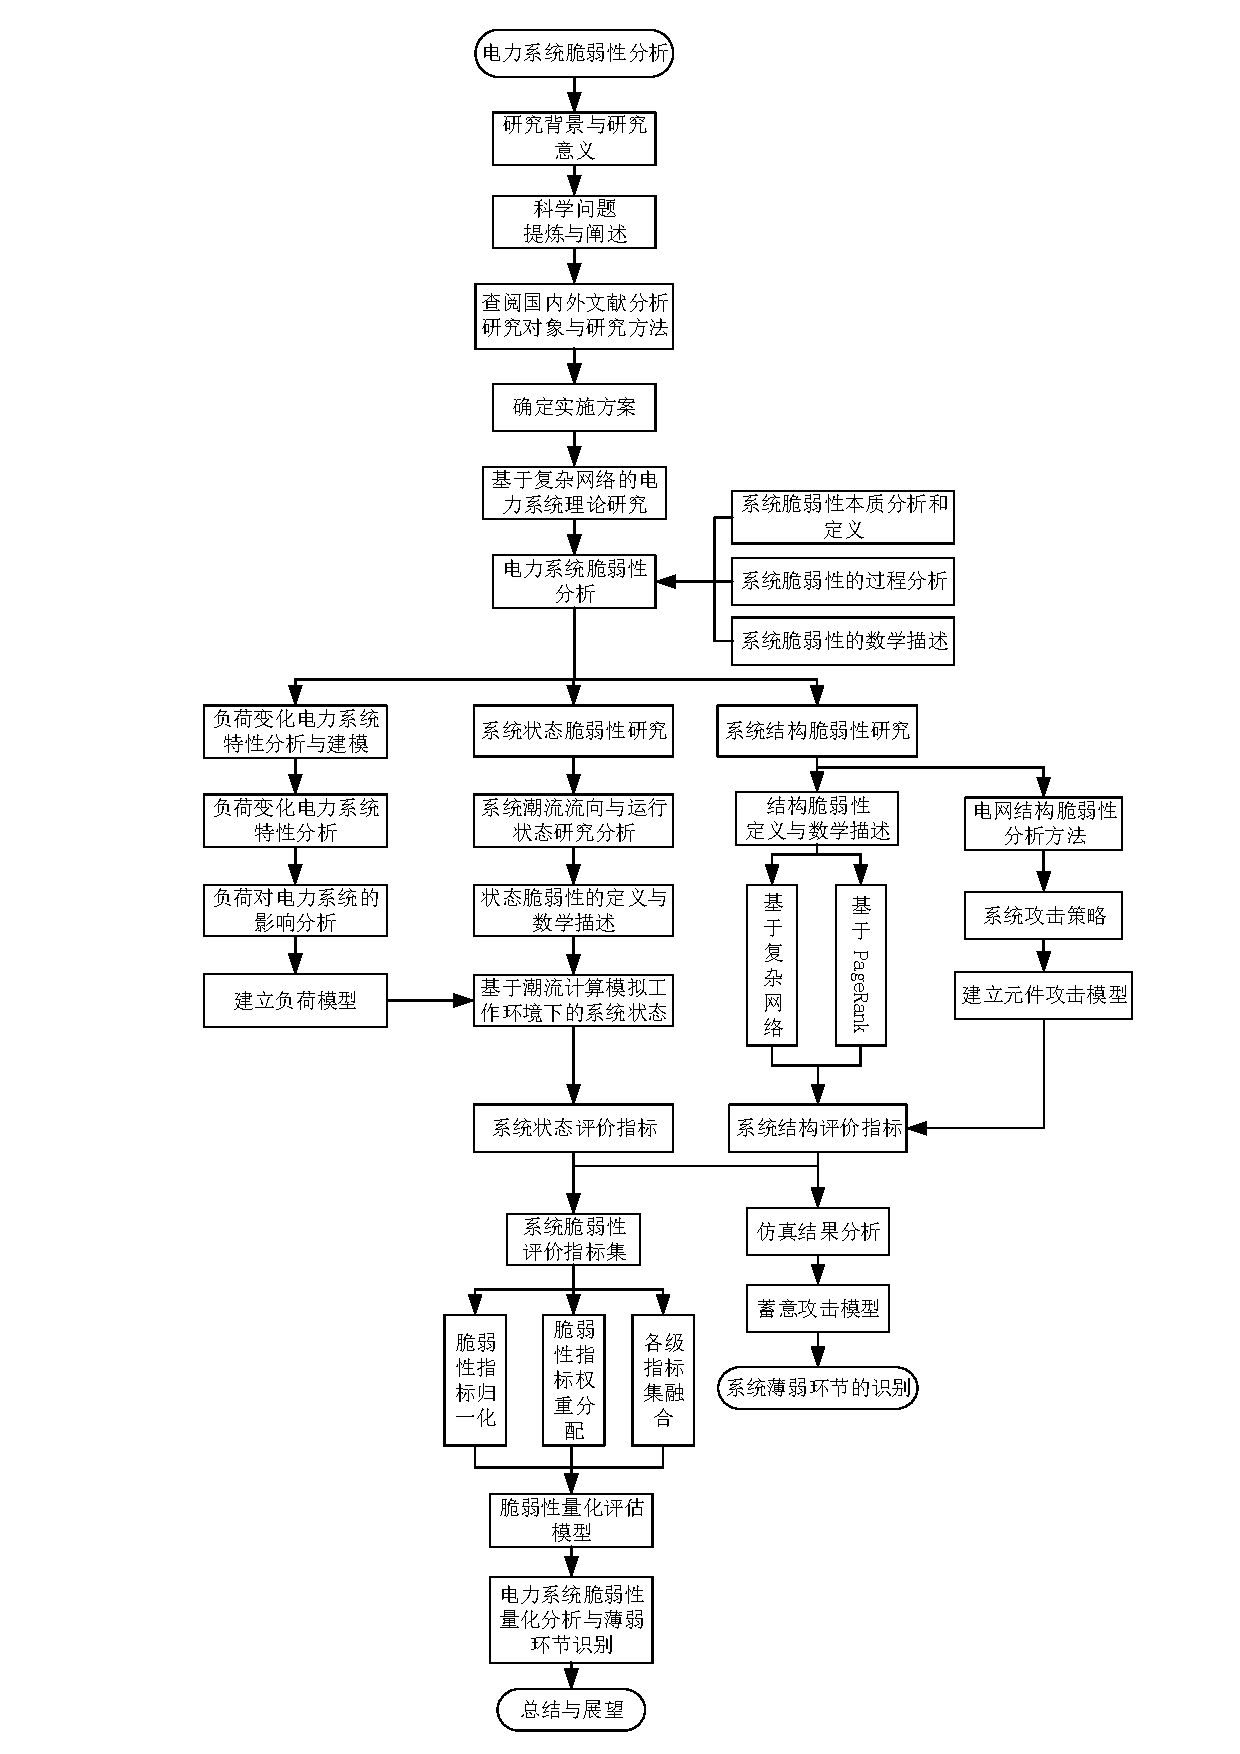
\includegraphics[height=23cm]{technicalRoute.pdf}
  \caption{技术路线图}
  \label{fig:technicalRoute}
\end{figure}
